%%%%%%%%%%%%%%%%%%%%%%%%%%%%%%%%%%%%%%%%%
% Masters/Doctoral Thesis 
% LaTeX Template
% Version 2.5 (27/8/17)
%
% This template was downloaded from:
% http://www.LaTeXTemplates.com
%
% Version 2.x major modifications by:
% Vel (vel@latextemplates.com)
%
% This template is based on a template by:
% Steve Gunn (http://users.ecs.soton.ac.uk/srg/softwaretools/document/templates/)
% Sunil Patel (http://www.sunilpatel.co.uk/thesis-template/)
%
% Template license:
% CC BY-NC-SA 3.0 (http://creativecommons.org/licenses/by-nc-sa/3.0/)
%
%%%%%%%%%%%%%%%%%%%%%%%%%%%%%%%%%%%%%%%%%

%----------------------------------------------------------------------------------------
%	PACKAGES AND OTHER DOCUMENT CONFIGURATIONS
%----------------------------------------------------------------------------------------

\documentclass[
11pt, % The default document font size, options: 10pt, 11pt, 12pt
%oneside, % Two side (alternating margins) for binding by default, uncomment to switch to one side
english, % ngerman for German
singlespacing, % Single line spacing, alternatives: onehalfspacing or doublespacing
%draft, % Uncomment to enable draft mode (no pictures, no links, overfull hboxes indicated)
%nolistspacing, % If the document is onehalfspacing or doublespacing, uncomment this to set spacing in lists to single
%liststotoc, % Uncomment to add the list of figures/tables/etc to the table of contents
%toctotoc, % Uncomment to add the main table of contents to the table of contents
%parskip, % Uncomment to add space between paragraphs
%nohyperref, % Uncomment to not load the hyperref package
headsepline, % Uncomment to get a line under the header
chapterinoneline, % Uncomment to place the chapter title next to the number on one line
%consistentlayout, % Uncomment to change the layout of the declaration, abstract and acknowledgements pages to match the default layout
oneside
]{MastersDoctoralThesis} % The class file specifying the document structure

\usepackage[utf8]{inputenc} % Required for inputting international characters
\usepackage[T1]{fontenc} % Output font encoding for international characters

\usepackage{mathpazo} % Use the Palatino font by default

\usepackage[backend=bibtex,style=authoryear,natbib=true]{biblatex} % Use the bibtex backend with the authoryear citation style (which resembles APA)

\addbibresource{example.bib} % The filename of the bibliography

\usepackage[autostyle=true]{csquotes} % Required to generate language-dependent quotes in the bibliography

\usepackage[toc,page]{appendix}

%----------------------------------------------------------------------------------------
%	MARGIN SETTINGS
%----------------------------------------------------------------------------------------

\geometry{
	paper=a4paper, % Change to letterpaper for US letter
	inner=2.5cm, % Inner margin
	outer=3.8cm, % Outer margin
	bindingoffset=.5cm, % Binding offset
	top=1.5cm, % Top margin
	bottom=1.5cm, % Bottom margin
	%showframe, % Uncomment to show how the type block is set on the page
}

%----------------------------------------------------------------------------------------
%	THESIS INFORMATION
%----------------------------------------------------------------------------------------

\thesistitle{Independent Study in Cluster Computing and Virtualization} % Your thesis title, this is used in the title and abstract, print it elsewhere with \ttitle
\supervisor{Dr. Alfred \textsc{McKinney}} % Your supervisor's name, this is used in the title page, print it elsewhere with \supname
\examiner{} % Your examiner's name, this is not currently used anywhere in the template, print it elsewhere with \examname
\degree{Independent Study} % Your degree name, this is used in the title page and abstract, print it elsewhere with \degreename
\author{\\Jay \textsc{Jain}\\ Blaise \textsc{Leonards}\\ Joshua \textsc{Schools}} % Your name, this is used in the title page and abstract, print it elsewhere with \authorname
\addresses{} % Your address, this is not currently used anywhere in the template, print it elsewhere with \addressname

\subject{Computer Science} % Your subject area, this is not currently used anywhere in the template, print it elsewhere with \subjectname
\keywords{parallel computing, cluster computing, Monte Carlo method} % Keywords for your thesis, this is not currently used anywhere in the template, print it elsewhere with \keywordnames
\university{\href{http://www.lsus.edu}{Louisiana State University - Shreveport}} % Your university's name and URL, this is used in the title page and abstract, print it elsewhere with \univname
\department{\href{http://www.lsus.edu/cs}{Department of Computer Science}} % Your department's name and URL, this is used in the title page and abstract, print it elsewhere with \deptname
\group{\href{http://researchgroup.university.com}{Research Group Name}} % Your research group's name and URL, this is used in the title page, print it elsewhere with \groupname
\faculty{\href{http://faculty.university.com}{Dr. Alfred McKinney}} % Your faculty's name and URL, this is used in the title page and abstract, print it elsewhere with \facname

\AtBeginDocument{
\hypersetup{pdftitle=\ttitle} % Set the PDF's title to your title
\hypersetup{pdfauthor=\authorname} % Set the PDF's author to your name
\hypersetup{pdfkeywords=\keywordnames} % Set the PDF's keywords to your keywords
}

\begin{document}

\frontmatter % Use roman page numbering style (i, ii, iii, iv...) for the pre-content pages

\pagestyle{plain} % Default to the plain heading style until the thesis style is called for the body content

%----------------------------------------------------------------------------------------
%	TITLE PAGE
%----------------------------------------------------------------------------------------

\begin{titlepage}
\begin{center}

\vspace*{.06\textheight}
{\scshape\LARGE \univname\par}\vspace{1.5cm} % University name
\textsc{\Large Independent Study}\\[0.5cm] % Thesis type

\HRule \\[0.4cm] % Horizontal line
{\huge \bfseries \ttitle\par}\vspace{0.4cm} % Thesis title
\HRule \\[1.5cm] % Horizontal line
 
\begin{minipage}[t]{0.4\textwidth}
\begin{flushleft} \large
\emph{Authors:}\\
\href{http://www.johnsmith.com}{\authorname} % Author name - remove the \href bracket to remove the link
\end{flushleft}
\end{minipage}
\begin{minipage}[t]{0.4\textwidth}
\begin{flushright} \large
\emph{Supervisor:} \\
\href{http://www.jamessmith.com}{\supname} % Supervisor name - remove the \href bracket to remove the link  
\end{flushright}
\end{minipage}\\[3cm]
 
\vfill

\large \textit{A document submitted in fulfillment of the requirements\\ for CSC 495 (Independent Study)}\\[0.3cm] % University requirement text
\textit{in the}\\[0.4cm]
%\groupname\\
\deptname\\[2cm] % Research group name and department name
 
\vfill

{\large \today}\\[4cm] % Date
%\includegraphics{Logo} % University/department logo - uncomment to place it
 
\vfill
\end{center}
\end{titlepage}

%----------------------------------------------------------------------------------------
%	DECLARATION PAGE
%----------------------------------------------------------------------------------------

%\begin{declaration}
%\addchaptertocentry{\authorshipname} % Add the declaration to the table of contents
%\noindent I, \authorname, declare that this thesis titled, \enquote{\ttitle} and the work presented in it are my own. I confirm that:
%
%\begin{itemize} 
%\item This work was done wholly or mainly while in candidature for a research degree at this University.
%\item Where any part of this thesis has previously been submitted for a degree or any other qualification at this University or any other institution, this has been clearly stated.
%\item Where I have consulted the published work of others, this is always clearly attributed.
%\item Where I have quoted from the work of others, the source is always given. With the exception of such quotations, this thesis is entirely my own work.
%\item I have acknowledged all main sources of help.
%\item Where the thesis is based on work done by myself jointly with others, I have made clear exactly what was done by others and what I have contributed myself.\\
%\end{itemize}
% 
%\noindent Signed:\\
%\rule[0.5em]{25em}{0.5pt} % This prints a line for the signature
% 
%\noindent Date:\\
%\rule[0.5em]{25em}{0.5pt} % This prints a line to write the date
%\end{declaration}
%
%\cleardoublepage

%----------------------------------------------------------------------------------------
%	QUOTATION PAGE
%----------------------------------------------------------------------------------------

\vspace*{0.2\textheight}

\noindent\enquote{\itshape For over a decade prophets have voiced the contention that the organization of a single computer has reached its limits and that truly significant advances can be made only by interconnection of a multiplicity of computers. }\bigbreak

\hfill Gene Amdahl

%----------------------------------------------------------------------------------------
%	ABSTRACT PAGE
%----------------------------------------------------------------------------------------

\begin{abstract}
\addchaptertocentry{\abstractname} % Add the abstract to the table of contents
Understanding the fundamentals of parallel computing in the age of big data is integral to a comprehensive computer science education. Over the course of the Fall 2017 semester, major mathematical and programming concepts were identified and implemented on a self-built Raspberry Pi cluster. The cluster consisted of a master node (Raspberry Pi 3) and four slave nodes (Raspberry Pi Zeros). Using the \texttt{Python} message passing interface (\texttt{mpi4py}), the value of pi was calculated using the Monte Carlo method at different iterations. The timing and accuracy of the calculated values of $\pi$ were compared using different parallel computing methods. In addition, the \texttt{Docker} virtualization interface was explored in order to understand the interrelation between parallel and cloud computing.    
\end{abstract}

%----------------------------------------------------------------------------------------
%	ACKNOWLEDGEMENTS
%----------------------------------------------------------------------------------------

\begin{acknowledgements}
\addchaptertocentry{\acknowledgementname} % Add the acknowledgements to the table of contents
The authors would like to thank Dr. McKinney for giving us the opportunity to participate in this independent study and his enduring kindness. We would also like to thank Mr. Phillip C.S.R. Kilgore for his words of encouragement and guidance through the project. Lastly, we would like to thank Dr. Cvek and Dr. Trutschl for allowing us to house our Raspberry Pi cluster in their laboratory.
\end{acknowledgements}

%----------------------------------------------------------------------------------------
%	LIST OF CONTENTS/FIGURES/TABLES PAGES
%----------------------------------------------------------------------------------------

\tableofcontents % Prints the main table of contents

%\listoffigures % Prints the list of figures

%\listoftables % Prints the list of tables

%----------------------------------------------------------------------------------------
%	ABBREVIATIONS
%----------------------------------------------------------------------------------------

\begin{abbreviations}{ll} % Include a list of abbreviations (a table of two columns)

\textbf{ARM} & \textbf{A}dvanced \textbf{R}ISC \textbf{M}achine\\
\textbf{ALU} & \textbf{Advanced} \textbf{Logic} \textbf{Unit}\\
\textbf{CCO} & \textbf{C}ollective \textbf{C}ommunication \textbf{O}peration\\
\textbf{DPM} & \textbf{D}ynamic \textbf{P}rocess \textbf{M}anagement\\
\textbf{MPI} & \textbf{M}essage \textbf{P}assing \textbf{I}nterface\\
\textbf{RMA} & \textbf{R}emote \textbf{M}emory \textbf{A}ccess\\
\textbf{RISC} & \textbf{R}educed \textbf{I}nstruction \textbf{S}et \textbf{C}omputer\\
\textbf{RPi} & \textbf{R}aspberry \textbf{Pi}\\
\textbf{SoC} & \textbf{S}ystem \textbf{o}n a \textbf{C}hip


\end{abbreviations}

%----------------------------------------------------------------------------------------
%	PHYSICAL CONSTANTS/OTHER DEFINITIONS
%----------------------------------------------------------------------------------------

%\begin{constants}{lr@{${}={}$}l} % The list of physical constants is a three column table
%
%% The \SI{}{} command is provided by the siunitx package, see its documentation for instructions on how to use it
%
%Speed of Light & $c_{0}$ & \SI{2.99792458e8}{\meter\per\second} (exact)\\
%%Constant Name & $Symbol$ & $Constant Value$ with units\\
%
%\end{constants}

%----------------------------------------------------------------------------------------
%	SYMBOLS
%----------------------------------------------------------------------------------------

%\begin{symbols}{lll} % Include a list of Symbols (a three column table)
%
%$a$ & distance & \si{\meter} \\
%$P$ & power & \si{\watt} (\si{\joule\per\second}) \\
%%Symbol & Name & Unit \\
%
%\addlinespace % Gap to separate the Roman symbols from the Greek
%
%$\omega$ & angular frequency & \si{\radian} \\
%
%\end{symbols}

%----------------------------------------------------------------------------------------
%	DEDICATION
%----------------------------------------------------------------------------------------

%\dedicatory{For/Dedicated to/To my\ldots} 

%----------------------------------------------------------------------------------------
%	THESIS CONTENT - CHAPTERS
%----------------------------------------------------------------------------------------

\mainmatter % Begin numeric (1,2,3...) page numbering

\pagestyle{thesis} % Return the page headers back to the "thesis" style

% Include the chapters of the thesis as separate files from the Chapters folder
% Uncomment the lines as you write the chapters

% Chapter 1

\chapter{Background} % Main chapter title

\label{Chapter1} % For referencing the chapter elsewhere, use \ref{Chapter1} 

%----------------------------------------------------------------------------------------

% Define some commands to keep the formatting separated from the content 
\newcommand{\keyword}[1]{\textbf{#1}}
\newcommand{\tabhead}[1]{\textbf{#1}}
\newcommand{\code}[1]{\texttt{#1}}
\newcommand{\file}[1]{\texttt{\bfseries#1}}
\newcommand{\option}[1]{\texttt{\itshape#1}}

%----------------------------------------------------------------------------------------

\section{Introduction}
	The idea for this independent study came from multiple conversations by the authors regarding the lack of a parallel or cluster computing course at the university. Subsequently, we have realized the importance of large scale processing in the age of big data. Understanding and analyzing big sets of data is a necessity in an age where almost all electronic devices (large and small) are connected to a network and feeding in trillions of data points per second. 
	
	We decided to utilize a set of Raspberry Pi computers as a small-scale example of a cluster computing platform. Initially, we thought that utilizing commodity hardware such as servers for our cluster would be the way to go. Unfortunately, we do not have access to such hardware, but after further research, we concluded that the Raspberry Pi would be sufficient to demonstrate concepts in parallel and cluster computing. 
	

%----------------------------------------------------------------------------------------

\section{Raspberry Pi }

	The Raspberry Pi is a low-cost, single-board computer that is capable of running light-weight GNU/Linux operating systems such as Raspbian. The Raspberry Pi utilizes the system on a chip (SoC) architecture in order to integrate components of the computer such as the microprocessor, graphics processing unit, and WiFi device. The Raspberry Pi is fairly easy to configure as there is a large, open-source community willing to help with setup issues. Additionally, the Raspberry Pi Foundation has put in a lot of effort to provide detailed and up-to-date documentation.

\subsection{ARM Architecture}

	The Raspberry Pi central processing unit utilizes the ARM Architecture developed by the ARM Holdings. The ARM architecture paradigm is extremely relevant as there have been over 100 billion devices produced (as of 2017) that utilize the ARM instructuction set architecture. Most handheld devices including iPads and gaming consoles utilize ARM cores.
	
	ARM, also known as Advanced RISC (Reduced Instruction Set Computing) Machine requires less transistors than x86 processors (usually found in personal computers) which make it an attractive candidate for embedded systems seeking to lower costs and energy consumption on devices. The ARM architecture supported only a core-bit width of 32, but the newest version of ARM, ARMv8 now supports both 32 and 64 bits as of 2011. Note, the Raspberry Pi utilizes ARMv7. ARMv7 adheres to the load/store architecture which separates instructions into memory access and ALU (Arithmetic Logic Unit) operations. Memory access is simply the process of transfering data from the memory to registers. ALU operations consist of the actual operations on the loaded memory. 

\subsection{Raspberry Pi 3}
	The Raspberry Pi 3 Model B consists of a quad-core 64-bit CPU with one gigabyte of RAM in the system on a chip configuration. Additionally, the RPi 3 is equipped with wireless LAN and Bluetooth capabilities. It is important to note that while the WiFi interface is speedy enough for basic internet usage, it does cause considerable bottlenecks when utilizing a parallel processing interface. In fact, the 802.11n WiFi speeds were clocked around 45 Mbits/second, while the USB Gigabit LAN clocked around 320 Mbits/second. Configuring USB Gigabit LAN with a Raspberry Pi cluster does take a considerable amount of time to configure as MAC addresses and USB devices have to be specifically assigned in order to ensure a functional RPi cluster. 

\subsection{Raspberry Pi Zero W}
	The Raspberry Pi Zero W is a lighter-weight WiFi-enabled version of the RPi 3. It has a 1GHz,single-core CPU with 512 MB of RAM. We utilized four RPi Zero W computers as our slave nodes. These nodes were utilized in order to carry out parallel processing while the RPi 3 was utilized as the master node which sent out jobs using the message passing interface (MPI). 

%----------------------------------------------------------------------------------------

\section{Message Passing Interface (MPI)}

	MPI is a standardized and portable parallel computing library usually used on supercomputers. The standards for MPI were first developed as parallel programs were being written in C, C++, and FORTRAN.Today, many other languages such as Python, R, and Java use wrapper classes in order to implement message passing interfaces written in C++ and FORTRAN.

\subsection{mpi4py}
	mpi4py is a message passing interface library for the Python programming language. We decided to use the Python programming language as it offers the implementation of high-level data structures with a dynamic typing and binding paradigm. Additionally, mpi4py has become one of the most utilized parallel computing libraries, thus there exists much online documentation and assistance. For instance, the devleopment of Python libraries such as NumPy make it easy to implement sometimes complex data structures such as arrays and dataframes in a user-friendly manner. Figure 1.1 shows some of the most basic parallel operations that mpi4py supports. The broadcast operation sends out the same operation to all slave nodes. The scatter operation sends out different operations to the worker nodes. The gather operation takes the output from the operation and sends it back to the master node. The reduction operation takes the output from the slave nodes and performs some type of operation. Please see code examples in Appendix A for a better understanding of MPI operations.
	
	
\begin{figure}
\centering
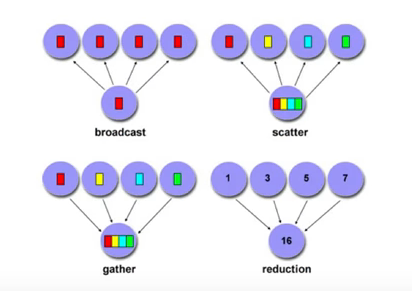
\includegraphics{Figures/mpi-diagram}
\decoRule
\caption[MPI Operations]{Four main supported MPI operations in mpi4py.}
\label{fig:MPI Operations}
\end{figure}


%----------------------------------------------------------------------------------------

\section{Docker}

Docker is an abstract, containerization system utilized for the automation and deployment of GNU/Linux operating systems.  Docker allows many single-images (known as containers) to run within one instance of Linux. This reduces the overhead of having to start and maintain many virtual machines.
    In the context of Docker, an image is a lightweight, executable package that has everything that is needed to run a piece of software, including code, libraries, environment variables, and configuration files. A container is the actual instance of an image when the image is executed on the operating system. The container runs independent of the host environment and can only access host files and networks if specified to do so. It is also important to note that containers run on the host machine’s kernel because the host kernel will produce better performance metrics than a virtual machine would. Figure 1.2 illustrates the aforementioned concepts.

\begin{figure}
\centering
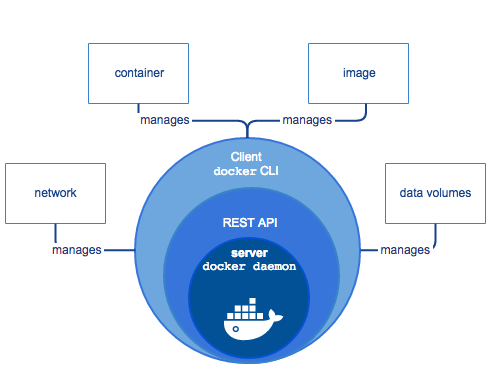
\includegraphics[scale=0.8]{Figures/docker-diagram}
\decoRule
\caption[Docker Architecture]{Illustration of Docker architecture.}
\label{fig:Docker Architecture}
\end{figure}



% Chapter Template

\chapter{Programs and Results} % Main chapter title

\label{Chapter 2} % Change X to a consecutive number; for referencing this chapter elsewhere, use \ref{ChapterX}

%----------------------------------------------------------------------------------------
%	SECTION 1
%----------------------------------------------------------------------------------------

\section{Calculating Pi }
To calculate the value of $\pi$ we decided to utilize the Monte Carlo method. The algorithm is as follows given that a circle and a square have a ratio of areas that is equal to $\pi$ / 4: \\
1. Draw a circle inscribed within a square. ( Figure \ref{fig:Monte-carlo} )\\
2. Randomly pick points within the area of the square.\\
3. Find the ratio of the number of points falling within the circle to the total of number of points.\\
4. The ratio of those points should be $\pi$ / 4.\\
5. To obtain the value of $\pi$ , multiply by 4.\\

The more random points (or "darts") thrown into the given area, the more accurate the value of pi will be. This is because as the numerator (number of points within the circle) and denominator (number of total points) gets larger, there will numbers with more decimal places. The following subsections will discuss the implementation of the above algorithm in three different MPI programming paradigms.

\begin{figure}
\centering
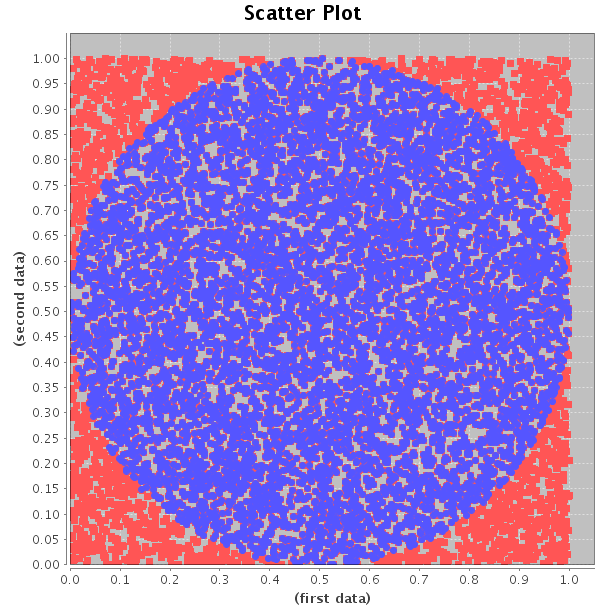
\includegraphics[scale=0.4]{Figures/monte-carlo}
\decoRule
\caption[Monte-Carlo Method]{Depiction of Monte Carlo method to calculate $\pi$ .}
\label{fig:Monte-carlo}
\end{figure}

\subsection {Collective Communication Operations}

One program that we used to calculate $\pi$ utilized the collective communication operations (CCO) method. The collective operation heavily relies on the communicator object which holds necessary information for assigning nodes their respective rank or job number. All processes (or in this case nodes) call the communicator object with the same arguments which ensures synchonization. Note, this is the most primitive form of parallel processing for our purposes as the problem is divided up and the slave  nodes perform the same operations. Susbequently, this is not the most efficient way to program a parallel job as not all job management should be hinged on the actual operation that needs to be completed.


\subsection {Dynamic Process Management}
With the advent of the MPI-2 standard, the implementation of dynamic processes has become much more common place with dynamic process management (DPM). DPM allows parent processes to create new child processes during runtime using spawn functionality. In addition, it can connect previously existing processes with each other with intercommunicator objects. The spawn function can create communicator objects with the original arguments or it can take new arguments.

	Although DPM offers much more flexibility and efficiency by handling bottlenecks, it requires much more code in order to implement. The code has to determine what jobs will be done by respective child process and how to handle multi-stage spawning. Multi-stage spawning occurs when two child process have to communicate with each other. The programmer has to determine if the child process will communicate with each other directly or if the parent node will act as the intercommunicator. See Figure \ref{fig:Multi-stage} for a visual representation of the parent job in blue with respective child jobs in green.
	
\begin{figure}
\centering
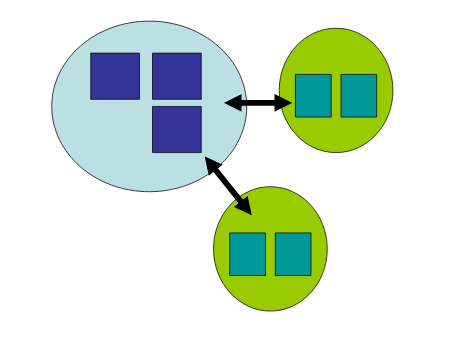
\includegraphics[scale=0.7]{Figures/multi-stage}
\decoRule
\caption[Multi-stage spawning]{An instance of multi-stage spawning.}
\label{fig:Multi-stage}
\end{figure}

\subsection {Remote Memory Access}
Remote memory access (RMA) is another feature implemented in MPI-2. RMA is highly convenient for parallel programming as it does not require the programmer to have send and receive calls for both sides of communication. For instance, all previous programs required an explicit call to send the data and an explicit call to receive the data. The RMA method allows one method call to send the data and at the same time it will automatically initiate a call to receive the data when necessary. This allows processes to act independently of each other when sending and receiving data. Traditionally, when a process sends a job or piece of data to another process or job, it has to wait until that information has been received. With RMA, once the information has been sent, the process is free to move onto its next task. For RMA to work, the process must specify a contiguous region of memory called a window that is open to all other processes. The other processes that are trying to access this space of memory must be aware of this window.


 
% Chapter Template

\chapter{Conclusion} % Main chapter title

\label{Chapter3} % Change X to a consecutive number; for referencing this chapter elsewhere, use \ref{ChapterX}

%----------------------------------------------------------------------------------------
%	SECTION 1
%----------------------------------------------------------------------------------------

\section{Conclusion}

After testing the Monte Carlo method to calcualte the value of $\pi$, the dynamic process management (DPM) method of programming calculated the value of $\pi$ the fastest with the least amount of deviation from the known value of $\pi$. Although DPM was superior to the other methods, it requires more lines of code and a higher-level of programming ability. 

Throughout the course of the semester, the authors have gained knowledge in parallel computing applications such as Python's \texttt{mpi4py} library and various mathematical methods utilized to improve throughput and efficiency in programming. In addition, the authors have gained experience in setting up cluster computing environments using GNU/Linux software and configuring networks in order to optimize interconnections between cluster computing nodes. 


%\include{Chapters/Chapter4} 
%\include{Chapters/Chapter5} 

%----------------------------------------------------------------------------------------
%	THESIS CONTENT - APPENDICES
%----------------------------------------------------------------------------------------

\appendix % Cue to tell LaTeX that the following "chapters" are Appendices

% Include the appendices of the thesis as separate files from the Appendices folder
% Uncomment the lines as you write the Appendices

% Appendix A

\chapter{Code Examples} % Main appendix title

\label{AppendixA} % For referencing this appendix elsewhere, use \ref{AppendixA}

\section{MPI Operations}

The color of links can be changed to your liking using:
%
%{\small\verb!\hypersetup{urlcolor=red}!}, or
%
%{\small\verb!\hypersetup{citecolor=green}!}, or
%
%{\small\verb!\hypersetup{allcolor=blue}!}.
%
%\noindent If you want to completely hide the links, you can use:
%
%{\small\verb!\hypersetup{allcolors=.}!}, or even better: 
%
%{\small\verb!\hypersetup{hidelinks}!}.
%
%\noindent If you want to have obvious links in the PDF but not the printed text, use:
%
%{\small\verb!\hypersetup{colorlinks=false}!}.

\subsection {Broadcast Example}
\label{appendix:broadcast}
\begin{verbatim}

from mpi4py import MPI
comm = MPI.COMM_WORLD
rank = comm.Get_rank()

if rank == 0:
	data = {'key1' : [7, 2.72, 2+3j],'key2' : ( 'abc', 'xyz')}
	print 'Broadcasting...',data
else:
	data = None
	
data = comm.bcast(data, root=0)
print 'Broadcasting...',data

\end{verbatim}

Output:

\begin{verbatim}

\end{verbatim}

\subsection {Scatter Example}
\label{appendix:scatter}
\begin{verbatim}
from mpi4py import MPI
comm = MPI.COMM_WORLD
size = comm.Get_size()
rank = comm.Get_rank()

if rank == 0:
	data = [(i+1)**2 for i in range(size)]
else:
	data = None

data = comm.scatter(data, root=0)
assert data == (rank+1)**2

\end{verbatim}

Output:

\begin{verbatim}

\end{verbatim}

\subsection {Gather Example}
\label{appendix:gather}

\begin{verbatim}
from mpi4py import MPI

comm = MPI.COMM_WORLD
size = comm.Get_size()
rank = comm.Get_rank()

data = (rank+1)**2
data = comm.gather(data, root=0)

if rank == 0:
	for i in range(size):
		assert data[i] == (i+1)**2
		print data[i],'from node',i
	print 'The final array:',data
else:
	assert data is None



\end{verbatim}

Output:

\begin{verbatim}

\end{verbatim}

\subsection {Reduction Example}

\label{appendix:reduction}
\begin{verbatim}
from mpi4py import MPI
import numpy
import sys
comm = MPI.COMM_SELF.Spawn(sys.executable,args=['cpi.py'],maxprocs=5)
N = numpy.array(100, 'i')
comm.Bcast([N, MPI.INT], root=MPI.ROOT)
PI = numpy.array(0.0, 'd')
comm.Reduce(None, [PI, MPI.DOUBLE],op=MPI.SUM, root=MPI.ROOT)
print (PI)
comm.Disconnect()


\end{verbatim}

Output:

\begin{verbatim}

\end{verbatim}
%\include{Appendices/AppendixB}
%\include{Appendices/AppendixC}

%----------------------------------------------------------------------------------------
%	BIBLIOGRAPHY
%----------------------------------------------------------------------------------------

\printbibliography[heading=bibintoc]

%----------------------------------------------------------------------------------------

\end{document}  
